\subsection{Intersymbol Interference}

The recieved signal can be represented as:

\begin{equation}
    \label{eqn:y-time}
    y[i] = \sum_{k=-\infty}^\infty a_k h[i-k] + w[i]
\end{equation}

The definition of autocorrelation coefficients:

\begin{equation}
    \label{eqn:auto-coeff}
    R_y[m] \triangleq E[y[i+m]y^*[i]]
\end{equation}

(\ref{eqn:expl-0}) Is a substitution of (\ref{eqn:y-time}) into (\ref{eqn:auto-coeff}) with the conjugate of y[i] and
$i$ substituted with $i+m$

\begin{equation}
    \label{eqn:expl-0}
    R_y[m] = E[(\sum_{k}a_kh[i+m-k]+w[i+m])(\sum_j a_j^* h_j^*[i-j]+w[i])]
\end{equation}

(\ref{eqn:expl-1}) this step shows that expected value of a vector multiplied by a conjugate is zero except when multiplied
by it's own conjugate.

\begin{equation}
    \label{eqn:expl-1}
    E[a_k a_j^*] =
    \begin{dcases}
        E_a \quad j=k \\
        0 \quad j \neq k
    \end{dcases}
\end{equation}

(\ref{eqn:expl-2}) Shows the principal of orthogonality where the expected value of the conjugate of the noise and $a_k$ is
zero a all points. This is due to the statistical independance of the two signals as AWGN is always statistically independent from all other
signals.

\begin{equation}
    \label{eqn:expl-2}
    E[a_k w^*[j]] = 0
\end{equation}

(\ref{eqn:expl-3}) this step shows that a vector multiplied by it's conjugate is zero except where multiplied by it's own
conjugate.

\begin{equation}
    \label{eqn:expl-3}
    E[w[j]w^*[k]] =
    \begin{dcases}
        \sigma_w^2 = \frac{N_0}{2} \quad j=k \\
        0 \quad j \neq k
    \end{dcases}
\end{equation}

(\ref{eqn:expl-4}) Is a simple substitution of the previous equations where $E_a$is from (\ref{eqn:expl-2}) The delta function is formed 
through (\ref{eqn:expl-3}), limiting the function to $\omega^2$ at 0 and 0 for all other values thus resulting in
$E[w[j]w^*[k]] = \frac{N_0}{2} \delta[m]$

\begin{equation}
    \label{eqn:expl-4}
    \therefore R_y[m] = \sum_k E_a h[i+m-k]h^*[i-k]+ \frac{N_0}{2}\delta [m]
\end{equation}

(\ref{eqn:expl-5}) simply sets $j=i-k$ to simplify the expression and sum over all j as well as using the linear properties of
the expected value to move $E_a$ out to the front of the sum as $E[aX] = aE[X]$\\

Hence,

\begin{equation}
    \label{eqn:expl-5}
    R_y[m] = E_a \sum_j h[m+j]h^*[j] + \frac{N_0}{2} \delta [m]
\end{equation}

\subsection{MMSE Equaliser}

Figure \ref{fig:equ-eye} shows the eye diagram of a signal after matched filtering but before equalisation. After equalisation
the eye diagram would appear to open due to the signal correction in equalisation. This corresponds with the reduction in the
symbol error probability as the eye diagram shows the distance between different amplitude levels. When there is not distinct levels
shown on the eye diagram this shows that accuratly dectecting the symbol is no longer possible. This is also shown on the scatter plots 
where the values at the sampling instant are shown. The data shown in Figure \ref{fig:equ-scatter} (b) also shows the seperation
between the symbol levels, indicationg that an accurate distinction could be made, compared to Figure \ref{fig:equ-scatter} (a)
where no accurate distinction can be made between the levels.

\begin{figure}[H]
    \begin{center}
        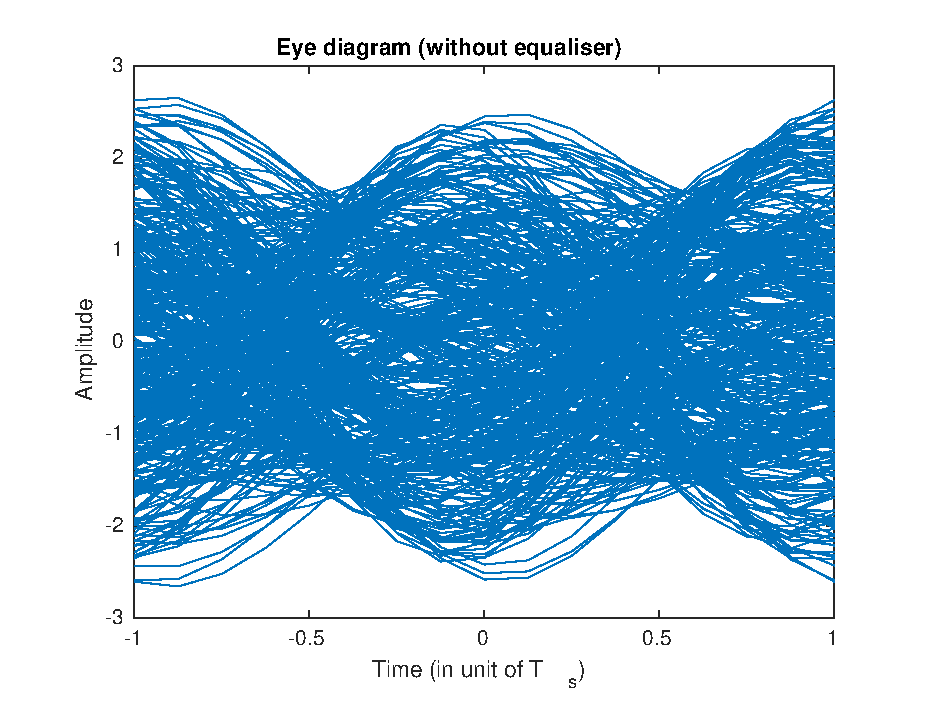
\includegraphics{Equaliser/eye}
    \end{center}
    \caption{Eye Diagram of a 4-PAM signal before equalisation}
    \label{fig:equ-eye}
\end{figure}

\begin{figure}[H]
    \begin{center}
        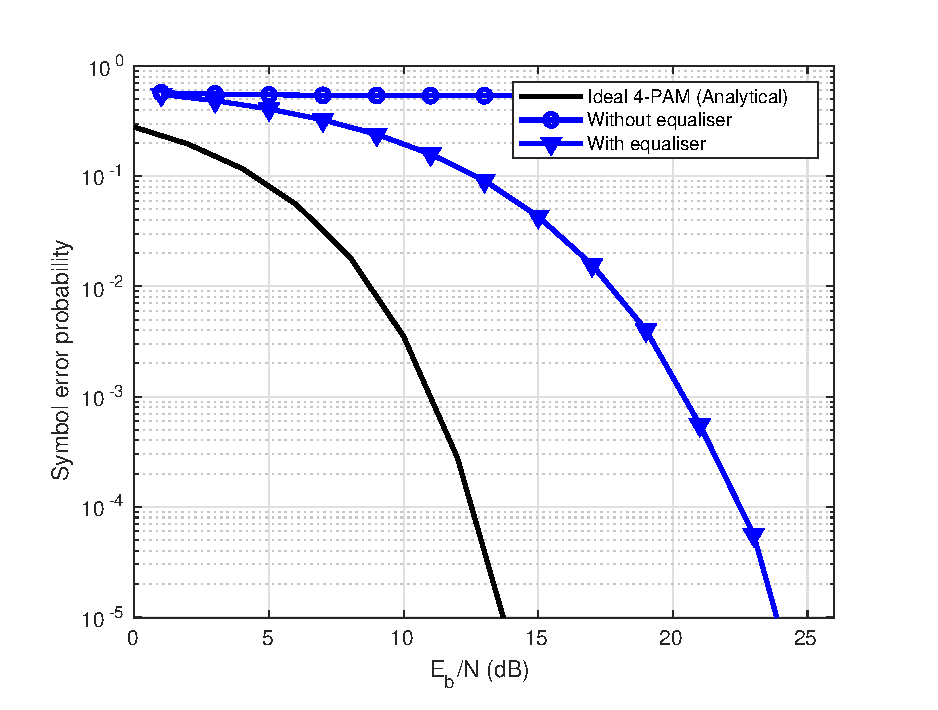
\includegraphics{Equaliser/ber}
    \end{center}
    \caption{SER comparison of a singal with and without equalisation}
    \label{fig:equ-ser}
\end{figure}

\begin{figure}[H]
    \begin{center}
        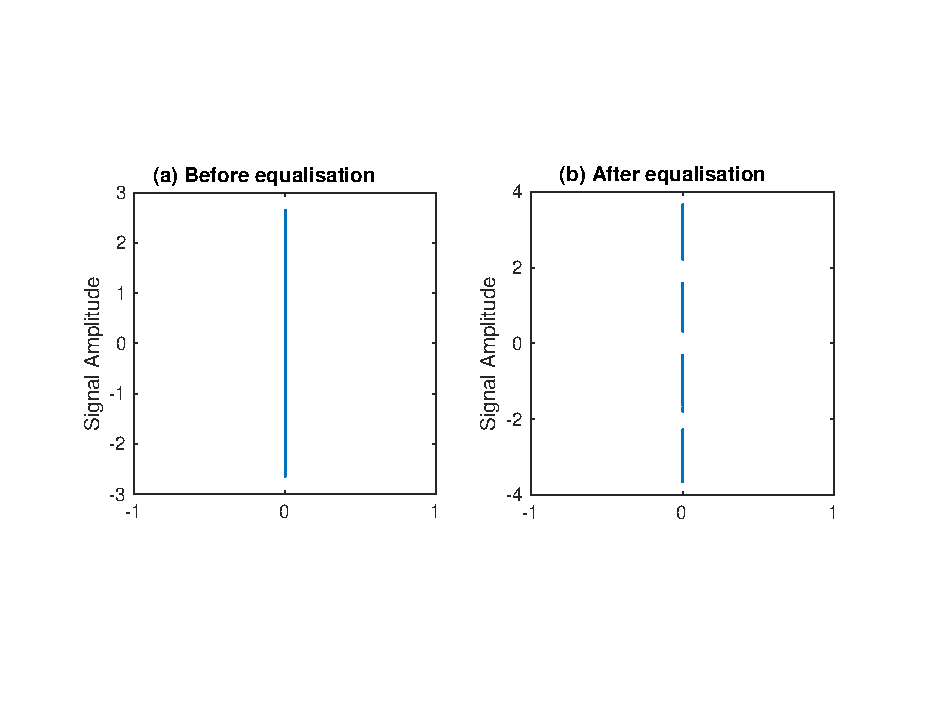
\includegraphics{Equaliser/scatter}
    \end{center}
    \caption{Before and after equalisation scatter plots showing the signal seperation after equalisation}
    \label{fig:equ-scatter}
\end{figure}

\subsection{Displaying a eye diagram with lab equipment}
To display an eye diagram on the ECE lab equipment the signal generator would have the clock output connected to the channel 1
input of the oscilloscope and the data output would be connected channel 2. The data generation on the signal generator would
be set to `RANDOM' this ensures a proper eye can be generated as it is not just the same data cycling. Next set an oscilloscope
trigger on the input to channel 1, this allows the oscilloscope to detect each period and know when to loop the signal on the screen.
Finally, the display persistance should be set to ininity to ensure that the past pulses are not removed from the screen so a proper
eye is formed.
